%!TEX encoding = UTF-8 Unicode

\documentclass[landscape]{book}
\usepackage[a3paper]{geometry}

\usepackage{verbatim}

\usepackage{hyperref}

\usepackage{tikz}

\usetikzlibrary{
  arrows,
  shapes.misc,% wg. rounded rectangle
  shapes.arrows,%
  matrix,%
  scopes,%
  shadows%
}

\tikzset{
  nonterminal/.style={
    % The shape:
    rectangle,
    % The size:
    minimum size=6mm,
    % The border:
    very thick,
    draw=red!50!black!50,         % 50% red and 50% black,
                                  % and that mixed with 50% white
    % The filling:
    top color=white,              % a shading that is white at the top...
    bottom color=red!50!black!20, % and something else at the bottom
    % Font
    font=\itshape\small
  },
  terminal/.style={
    % The shape:
    rounded rectangle,
    minimum size=6mm,
    % The rest
    very thick,draw=black!50,
    top color=white,bottom color=black!20,
    font=\ttfamily\small
  },
  firstPoint/.style={circle,>=stealth',thick,draw=black!50},
  point/.style={coordinate,>=stealth',thick,draw=black!50},
  tip/.style={->,shorten >=0.007pt},
  lastPoint/.style={rectangle,>=stealth',thick,draw=black!50},
  every join/.style={rounded corners}
}

\newcommand\nonTerminalSection[2]{\section{Nonterminal \texttt{#1}}\label{nt:#2}}
\newcommand\ruleSubsection[3]{\subsection{Component \texttt{#1}, in file \texttt{#2}, line #3}}
\newcommand\ruleMatrixColumnSeparation{3mm}
\newcommand\ruleMatrixRowSeparation{3mm}
\newcommand\nonTerminalSymbol[2]{\hyperref[nt:#2]{#1}}
\newcommand\startSymbol[2]{The start symbol is \hyperref[nt:#2]{#1}.}

\newcommand\nonTerminalSummaryStart{This is the alphabetical list of non terminal : }
\newcommand\nonTerminalSummary[2]{\hyperref[nt:#2]{#1}}
\newcommand\nonTerminalSummarySeparator{, }
\newcommand\nonTerminalSummaryEnd{.\\}

\begin{document}

\title{\Huge{Grammar \texttt{templateGrammar}}}
\date \today 

\maketitle

\startSymbol{template\_parser\_start\_symbol}{9}

\nonTerminalSummaryStart \nonTerminalSummary{expression}{0}\nonTerminalSummarySeparator \nonTerminalSummary{factor}{5}\nonTerminalSummarySeparator \nonTerminalSummary{for\_instruction\_element}{10}\nonTerminalSummarySeparator \nonTerminalSummary{for\_instruction\_enumerated\_object}{11}\nonTerminalSummarySeparator \nonTerminalSummary{output\_expression\_list}{7}\nonTerminalSummarySeparator \nonTerminalSummary{primary}{6}\nonTerminalSummarySeparator \nonTerminalSummary{relation\_factor}{2}\nonTerminalSummarySeparator \nonTerminalSummary{relation\_term}{1}\nonTerminalSummarySeparator \nonTerminalSummary{simple\_expression}{3}\nonTerminalSummarySeparator \nonTerminalSummary{switch\_case}{12}\nonTerminalSummarySeparator \nonTerminalSummary{template\_instruction}{8}\nonTerminalSummarySeparator \nonTerminalSummary{template\_parser\_start\_symbol}{9}\nonTerminalSummarySeparator \nonTerminalSummary{term}{4}\nonTerminalSummaryEnd \nonTerminalSection{expression}{0}

\ruleSubsection{templateSyntax}{templateSyntax}{26}

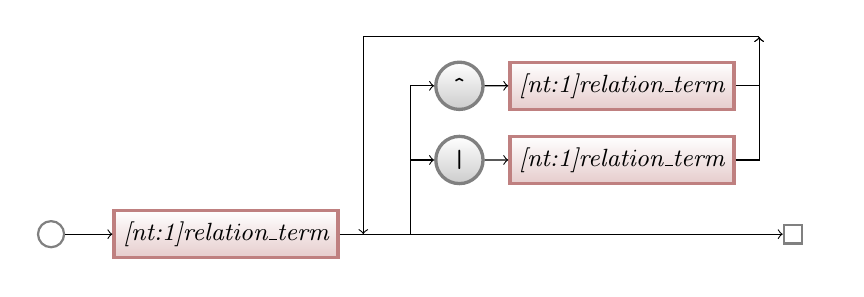
\begin{tikzpicture}
  \matrix[column sep=\ruleMatrixColumnSeparation, row sep=\ruleMatrixRowSeparation] {
    & & & & & & & & \node (p3-8) [point] {}; & \\
    & & & & & & \node (p2-6) [terminal] {\verb=^=}; & \node (p2-7) [nonterminal] {\nonTerminalSymbol{relation\_term}{1}}; & \\
    & & & & & & \node (p1-6) [terminal] {|}; & \node (p1-7) [nonterminal] {\nonTerminalSymbol{relation\_term}{1}}; & \\
    \node (P0start) [firstPoint] {}; & & \node (p0-2) [nonterminal] {\nonTerminalSymbol{relation\_term}{1}}; & \node (p0-3) [point] {}; & \node (p0-4) [point] {}; & \node (p0-5) [point] {}; & & & & \node (p0-9) [lastPoint] {}; & \\
  };
  \draw[->] (P0start) -- (p0-2) ;
  \draw (p0-2) -- (p0-4) ;
  \draw[->] (p0-5) |- (p1-6) ;
  \draw[->] (p1-6) -- (p1-7) ;
  \draw[->] (p0-5) |- (p2-6) ;
  \draw[->] (p2-6) -- (p2-7) ;
  \draw[->] (p3-8) -| (p0-3) ;
  \draw[->] (p1-7) -| (p3-8) ;
  \draw[->] (p2-7) -| (p3-8) ;
  \draw[->] (p0-4) -- (p0-9) ;
\end{tikzpicture}

\nonTerminalSection{factor}{5}

\ruleSubsection{templateSyntax}{templateSyntax}{202}

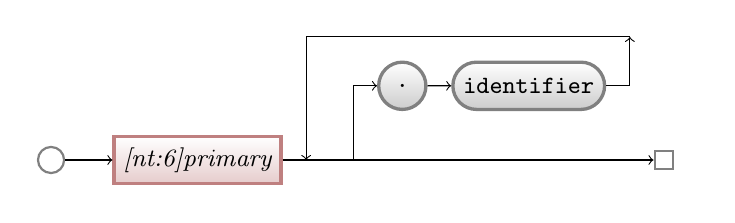
\begin{tikzpicture}
  \matrix[column sep=\ruleMatrixColumnSeparation, row sep=\ruleMatrixRowSeparation] {
    & & & & & & & & \node (p2-8) [point] {}; & \\
    & & & & & & \node (p1-6) [terminal] {.}; & \node (p1-7) [terminal] {identifier}; & \\
    \node (P0start) [firstPoint] {}; & & \node (p0-2) [nonterminal] {\nonTerminalSymbol{primary}{6}}; & \node (p0-3) [point] {}; & \node (p0-4) [point] {}; & \node (p0-5) [point] {}; & & & & \node (p0-9) [lastPoint] {}; & \\
  };
  \draw[->] (P0start) -- (p0-2) ;
  \draw (p0-2) -- (p0-4) ;
  \draw[->] (p0-5) |- (p1-6) ;
  \draw[->] (p1-6) -- (p1-7) ;
  \draw[->] (p2-8) -| (p0-3) ;
  \draw[->] (p1-7) -| (p2-8) ;
  \draw[->] (p0-4) -- (p0-9) ;
\end{tikzpicture}

\ruleSubsection{templateSyntax}{templateSyntax}{218}

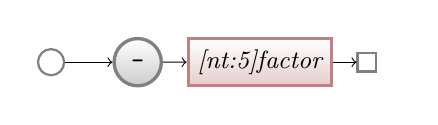
\begin{tikzpicture}
  \matrix[column sep=\ruleMatrixColumnSeparation, row sep=\ruleMatrixRowSeparation] {
    \node (P0start) [firstPoint] {}; & & \node (p0-2) [terminal] {-}; & \node (p0-3) [nonterminal] {\nonTerminalSymbol{factor}{5}}; & \node (p0-4) [lastPoint] {}; & \\
  };
  \draw[->] (P0start) -- (p0-2) ;
  \draw[->] (p0-2) -- (p0-3) ;
  \draw[->] (p0-3) -- (p0-4) ;
\end{tikzpicture}

\ruleSubsection{templateSyntax}{templateSyntax}{232}

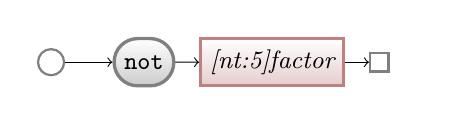
\begin{tikzpicture}
  \matrix[column sep=\ruleMatrixColumnSeparation, row sep=\ruleMatrixRowSeparation] {
    \node (P0start) [firstPoint] {}; & & \node (p0-2) [terminal] {not}; & \node (p0-3) [nonterminal] {\nonTerminalSymbol{factor}{5}}; & \node (p0-4) [lastPoint] {}; & \\
  };
  \draw[->] (P0start) -- (p0-2) ;
  \draw[->] (p0-2) -- (p0-3) ;
  \draw[->] (p0-3) -- (p0-4) ;
\end{tikzpicture}

\ruleSubsection{templateSyntax}{templateSyntax}{246}

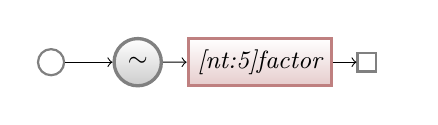
\begin{tikzpicture}
  \matrix[column sep=\ruleMatrixColumnSeparation, row sep=\ruleMatrixRowSeparation] {
    \node (P0start) [firstPoint] {}; & & \node (p0-2) [terminal] {$\sim$}; & \node (p0-3) [nonterminal] {\nonTerminalSymbol{factor}{5}}; & \node (p0-4) [lastPoint] {}; & \\
  };
  \draw[->] (P0start) -- (p0-2) ;
  \draw[->] (p0-2) -- (p0-3) ;
  \draw[->] (p0-3) -- (p0-4) ;
\end{tikzpicture}

\nonTerminalSection{for\_instruction\_element}{10}

\ruleSubsection{templateSyntax}{template-for-instruction}{31}

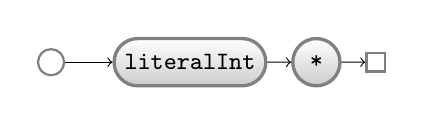
\begin{tikzpicture}
  \matrix[column sep=\ruleMatrixColumnSeparation, row sep=\ruleMatrixRowSeparation] {
    \node (P0start) [firstPoint] {}; & & \node (p0-2) [terminal] {literalInt}; & \node (p0-3) [terminal] {*}; & \node (p0-4) [lastPoint] {}; & \\
  };
  \draw[->] (P0start) -- (p0-2) ;
  \draw[->] (p0-2) -- (p0-3) ;
  \draw[->] (p0-3) -- (p0-4) ;
\end{tikzpicture}

\ruleSubsection{templateSyntax}{template-for-instruction}{46}

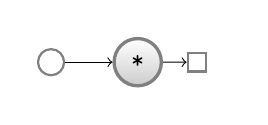
\begin{tikzpicture}
  \matrix[column sep=\ruleMatrixColumnSeparation, row sep=\ruleMatrixRowSeparation] {
    \node (P0start) [firstPoint] {}; & & \node (p0-2) [terminal] {*}; & \node (p0-3) [lastPoint] {}; & \\
  };
  \draw[->] (P0start) -- (p0-2) ;
  \draw[->] (p0-2) -- (p0-3) ;
\end{tikzpicture}

\ruleSubsection{templateSyntax}{template-for-instruction}{53}

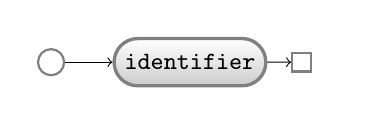
\begin{tikzpicture}
  \matrix[column sep=\ruleMatrixColumnSeparation, row sep=\ruleMatrixRowSeparation] {
    \node (P0start) [firstPoint] {}; & & \node (p0-2) [terminal] {identifier}; & \node (p0-3) [lastPoint] {}; & \\
  };
  \draw[->] (P0start) -- (p0-2) ;
  \draw[->] (p0-2) -- (p0-3) ;
\end{tikzpicture}

\nonTerminalSection{for\_instruction\_enumerated\_object}{11}

\ruleSubsection{templateSyntax}{template-for-instruction}{60}

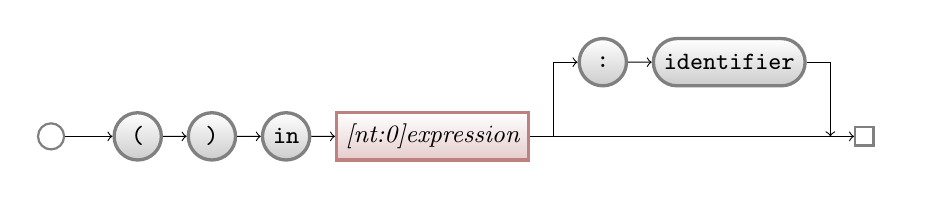
\begin{tikzpicture}
  \matrix[column sep=\ruleMatrixColumnSeparation, row sep=\ruleMatrixRowSeparation] {
    & & & & & & & \node (p1-7) [terminal] {:}; & \node (p1-8) [terminal] {identifier}; & \\
    \node (P0start) [firstPoint] {}; & & \node (p0-2) [terminal] {(}; & \node (p0-3) [terminal] {)}; & \node (p0-4) [terminal] {in}; & \node (p0-5) [nonterminal] {\nonTerminalSymbol{expression}{0}}; & \node (p0-6) [point] {}; & \node (p0-7) [point] {}; & & \node (p0-9) [point] {}; & \node (p0-10) [lastPoint] {}; & \\
  };
  \draw[->] (P0start) -- (p0-2) ;
  \draw[->] (p0-2) -- (p0-3) ;
  \draw[->] (p0-3) -- (p0-4) ;
  \draw[->] (p0-4) -- (p0-5) ;
  \draw (p0-5) -- (p0-7) ;
  \draw[->] (p0-6) |- (p1-7) ;
  \draw[->] (p1-7) -- (p1-8) ;
  \draw (p0-7) -- (p0-9) ;
  \draw[->] (p1-8) -| (p0-9) ;
  \draw[->] (p0-9) -- (p0-10) ;
\end{tikzpicture}

\ruleSubsection{templateSyntax}{template-for-instruction}{81}

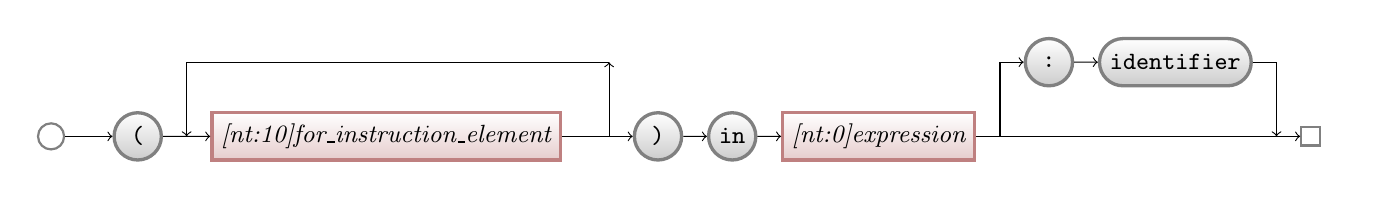
\begin{tikzpicture}
  \matrix[column sep=\ruleMatrixColumnSeparation, row sep=\ruleMatrixRowSeparation] {
    & & & & & & \node (p1-6) [point] {}; & & & & & \node (p1-11) [terminal] {:}; & \node (p1-12) [terminal] {identifier}; & \\
    \node (P0start) [firstPoint] {}; & & \node (p0-2) [terminal] {(}; & \node (p0-3) [point] {}; & \node (p0-4) [nonterminal] {\nonTerminalSymbol{for\_instruction\_element}{10}}; & \node (p0-5) [point] {}; & & \node (p0-7) [terminal] {)}; & \node (p0-8) [terminal] {in}; & \node (p0-9) [nonterminal] {\nonTerminalSymbol{expression}{0}}; & \node (p0-10) [point] {}; & \node (p0-11) [point] {}; & & \node (p0-13) [point] {}; & \node (p0-14) [lastPoint] {}; & \\
  };
  \draw[->] (P0start) -- (p0-2) ;
  \draw[->] (p0-2) -- (p0-4) ;
  \draw[->] (p1-6) -| (p0-3) ;
  \draw[->] (p0-5) -| (p1-6) ;
  \draw[->] (p0-4) -- (p0-7) ;
  \draw[->] (p0-7) -- (p0-8) ;
  \draw[->] (p0-8) -- (p0-9) ;
  \draw (p0-9) -- (p0-11) ;
  \draw[->] (p0-10) |- (p1-11) ;
  \draw[->] (p1-11) -- (p1-12) ;
  \draw (p0-11) -- (p0-13) ;
  \draw[->] (p1-12) -| (p0-13) ;
  \draw[->] (p0-13) -- (p0-14) ;
\end{tikzpicture}

\nonTerminalSection{output\_expression\_list}{7}

\ruleSubsection{templateSyntax}{templateSyntax}{477}

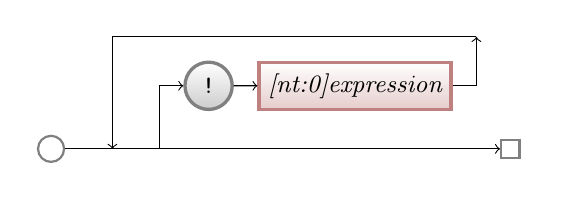
\begin{tikzpicture}
  \matrix[column sep=\ruleMatrixColumnSeparation, row sep=\ruleMatrixRowSeparation] {
    & & & & & & & \node (p2-7) [point] {}; & \\
    & & & & & \node (p1-5) [terminal] {!}; & \node (p1-6) [nonterminal] {\nonTerminalSymbol{expression}{0}}; & \\
    \node (P0start) [firstPoint] {}; & & \node (p0-2) [point] {}; & \node (p0-3) [point] {}; & \node (p0-4) [point] {}; & & & & \node (p0-8) [lastPoint] {}; & \\
  };
  \draw (P0start) -- (p0-3) ;
  \draw[->] (p0-4) |- (p1-5) ;
  \draw[->] (p1-5) -- (p1-6) ;
  \draw[->] (p2-7) -| (p0-2) ;
  \draw[->] (p1-6) -| (p2-7) ;
  \draw[->] (p0-3) -- (p0-8) ;
\end{tikzpicture}

\nonTerminalSection{primary}{6}

\ruleSubsection{templateSyntax}{templateSyntax}{261}

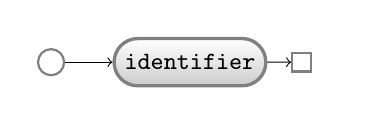
\begin{tikzpicture}
  \matrix[column sep=\ruleMatrixColumnSeparation, row sep=\ruleMatrixRowSeparation] {
    \node (P0start) [firstPoint] {}; & & \node (p0-2) [terminal] {identifier}; & \node (p0-3) [lastPoint] {}; & \\
  };
  \draw[->] (P0start) -- (p0-2) ;
  \draw[->] (p0-2) -- (p0-3) ;
\end{tikzpicture}

\ruleSubsection{templateSyntax}{templateSyntax}{272}

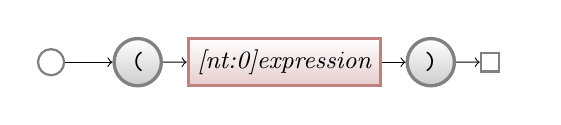
\begin{tikzpicture}
  \matrix[column sep=\ruleMatrixColumnSeparation, row sep=\ruleMatrixRowSeparation] {
    \node (P0start) [firstPoint] {}; & & \node (p0-2) [terminal] {(}; & \node (p0-3) [nonterminal] {\nonTerminalSymbol{expression}{0}}; & \node (p0-4) [terminal] {)}; & \node (p0-5) [lastPoint] {}; & \\
  };
  \draw[->] (P0start) -- (p0-2) ;
  \draw[->] (p0-2) -- (p0-3) ;
  \draw[->] (p0-3) -- (p0-4) ;
  \draw[->] (p0-4) -- (p0-5) ;
\end{tikzpicture}

\ruleSubsection{templateSyntax}{templateSyntax}{284}

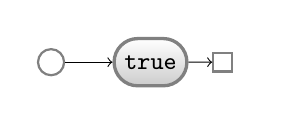
\begin{tikzpicture}
  \matrix[column sep=\ruleMatrixColumnSeparation, row sep=\ruleMatrixRowSeparation] {
    \node (P0start) [firstPoint] {}; & & \node (p0-2) [terminal] {true}; & \node (p0-3) [lastPoint] {}; & \\
  };
  \draw[->] (P0start) -- (p0-2) ;
  \draw[->] (p0-2) -- (p0-3) ;
\end{tikzpicture}

\ruleSubsection{templateSyntax}{templateSyntax}{295}

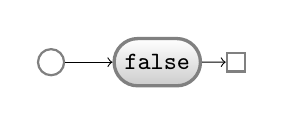
\begin{tikzpicture}
  \matrix[column sep=\ruleMatrixColumnSeparation, row sep=\ruleMatrixRowSeparation] {
    \node (P0start) [firstPoint] {}; & & \node (p0-2) [terminal] {false}; & \node (p0-3) [lastPoint] {}; & \\
  };
  \draw[->] (P0start) -- (p0-2) ;
  \draw[->] (p0-2) -- (p0-3) ;
\end{tikzpicture}

\ruleSubsection{templateSyntax}{templateSyntax}{306}

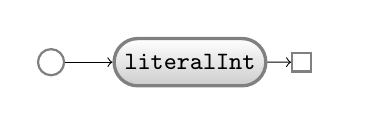
\begin{tikzpicture}
  \matrix[column sep=\ruleMatrixColumnSeparation, row sep=\ruleMatrixRowSeparation] {
    \node (P0start) [firstPoint] {}; & & \node (p0-2) [terminal] {literalInt}; & \node (p0-3) [lastPoint] {}; & \\
  };
  \draw[->] (P0start) -- (p0-2) ;
  \draw[->] (p0-2) -- (p0-3) ;
\end{tikzpicture}

\ruleSubsection{templateSyntax}{templateSyntax}{317}

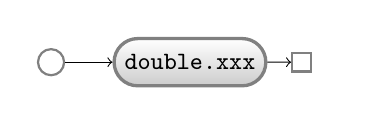
\begin{tikzpicture}
  \matrix[column sep=\ruleMatrixColumnSeparation, row sep=\ruleMatrixRowSeparation] {
    \node (P0start) [firstPoint] {}; & & \node (p0-2) [terminal] {double.xxx}; & \node (p0-3) [lastPoint] {}; & \\
  };
  \draw[->] (P0start) -- (p0-2) ;
  \draw[->] (p0-2) -- (p0-3) ;
\end{tikzpicture}

\ruleSubsection{templateSyntax}{templateSyntax}{329}

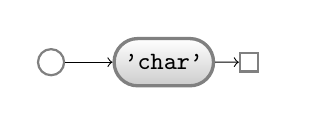
\begin{tikzpicture}
  \matrix[column sep=\ruleMatrixColumnSeparation, row sep=\ruleMatrixRowSeparation] {
    \node (P0start) [firstPoint] {}; & & \node (p0-2) [terminal] {'char'}; & \node (p0-3) [lastPoint] {}; & \\
  };
  \draw[->] (P0start) -- (p0-2) ;
  \draw[->] (p0-2) -- (p0-3) ;
\end{tikzpicture}

\ruleSubsection{templateSyntax}{templateSyntax}{340}

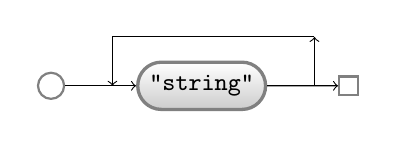
\begin{tikzpicture}
  \matrix[column sep=\ruleMatrixColumnSeparation, row sep=\ruleMatrixRowSeparation] {
    & & & & & \node (p1-5) [point] {}; & \\
    \node (P0start) [firstPoint] {}; & & \node (p0-2) [point] {}; & \node (p0-3) [terminal] {"string"}; & \node (p0-4) [point] {}; & & \node (p0-6) [lastPoint] {}; & \\
  };
  \draw[->] (P0start) -- (p0-3) ;
  \draw[->] (p1-5) -| (p0-2) ;
  \draw[->] (p0-4) -| (p1-5) ;
  \draw[->] (p0-3) -- (p0-6) ;
\end{tikzpicture}

\ruleSubsection{templateSyntax}{templateSyntax}{362}

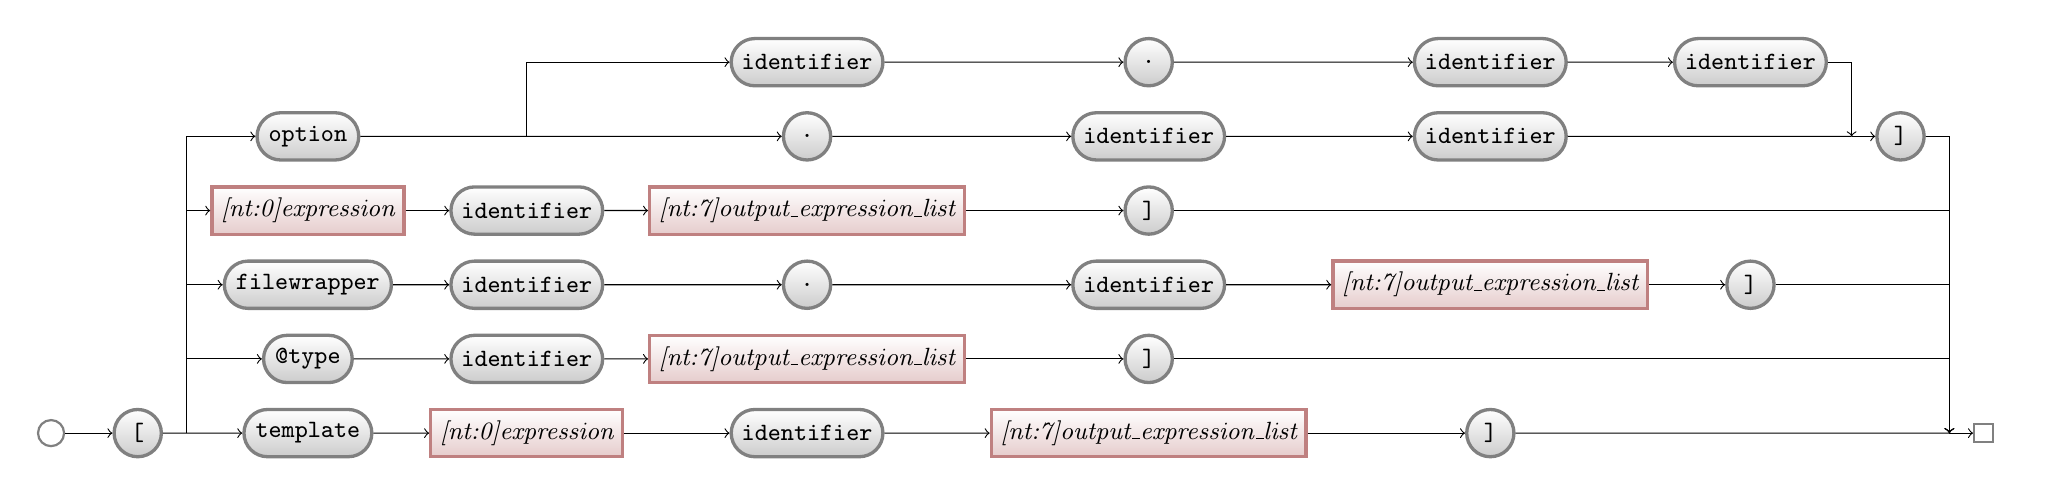
\begin{tikzpicture}
  \matrix[column sep=\ruleMatrixColumnSeparation, row sep=\ruleMatrixRowSeparation] {
    & & & & & & \node (p5-6) [terminal] {identifier}; & \node (p5-7) [terminal] {.}; & \node (p5-8) [terminal] {identifier}; & \node (p5-9) [terminal] {identifier}; & \\
    & & & & \node (p4-4) [terminal] {option}; & \node (p4-5) [point] {}; & \node (p4-6) [terminal] {.}; & \node (p4-7) [terminal] {identifier}; & \node (p4-8) [terminal] {identifier}; & & \node (p4-10) [point] {}; & \node (p4-11) [terminal] {]}; & \\
    & & & & \node (p3-4) [nonterminal] {\nonTerminalSymbol{expression}{0}}; & \node (p3-5) [terminal] {identifier}; & \node (p3-6) [nonterminal] {\nonTerminalSymbol{output\_expression\_list}{7}}; & \node (p3-7) [terminal] {]}; & \\
    & & & & \node (p2-4) [terminal] {filewrapper}; & \node (p2-5) [terminal] {identifier}; & \node (p2-6) [terminal] {.}; & \node (p2-7) [terminal] {identifier}; & \node (p2-8) [nonterminal] {\nonTerminalSymbol{output\_expression\_list}{7}}; & \node (p2-9) [terminal] {]}; & \\
    & & & & \node (p1-4) [terminal] {@type}; & \node (p1-5) [terminal] {identifier}; & \node (p1-6) [nonterminal] {\nonTerminalSymbol{output\_expression\_list}{7}}; & \node (p1-7) [terminal] {]}; & \\
    \node (P0start) [firstPoint] {}; & & \node (p0-2) [terminal] {[}; & \node (p0-3) [point] {}; & \node (p0-4) [terminal] {template}; & \node (p0-5) [nonterminal] {\nonTerminalSymbol{expression}{0}}; & \node (p0-6) [terminal] {identifier}; & \node (p0-7) [nonterminal] {\nonTerminalSymbol{output\_expression\_list}{7}}; & \node (p0-8) [terminal] {]}; & & & & \node (p0-12) [point] {}; & \node (p0-13) [lastPoint] {}; & \\
  };
  \draw[->] (P0start) -- (p0-2) ;
  \draw[->] (p0-2) -- (p0-4) ;
  \draw[->] (p0-4) -- (p0-5) ;
  \draw[->] (p0-5) -- (p0-6) ;
  \draw[->] (p0-6) -- (p0-7) ;
  \draw[->] (p0-7) -- (p0-8) ;
  \draw[->] (p0-3) |- (p1-4) ;
  \draw[->] (p1-4) -- (p1-5) ;
  \draw[->] (p1-5) -- (p1-6) ;
  \draw[->] (p1-6) -- (p1-7) ;
  \draw[->] (p0-3) |- (p2-4) ;
  \draw[->] (p2-4) -- (p2-5) ;
  \draw[->] (p2-5) -- (p2-6) ;
  \draw[->] (p2-6) -- (p2-7) ;
  \draw[->] (p2-7) -- (p2-8) ;
  \draw[->] (p2-8) -- (p2-9) ;
  \draw[->] (p0-3) |- (p3-4) ;
  \draw[->] (p3-4) -- (p3-5) ;
  \draw[->] (p3-5) -- (p3-6) ;
  \draw[->] (p3-6) -- (p3-7) ;
  \draw[->] (p0-3) |- (p4-4) ;
  \draw[->] (p4-4) -- (p4-6) ;
  \draw[->] (p4-6) -- (p4-7) ;
  \draw[->] (p4-7) -- (p4-8) ;
  \draw[->] (p4-5) |- (p5-6) ;
  \draw[->] (p5-6) -- (p5-7) ;
  \draw[->] (p5-7) -- (p5-8) ;
  \draw[->] (p5-8) -- (p5-9) ;
  \draw (p4-8) -- (p4-10) ;
  \draw[->] (p5-9) -| (p4-10) ;
  \draw[->] (p4-10) -- (p4-11) ;
  \draw (p0-8) -- (p0-12) ;
  \draw[->] (p1-7) -| (p0-12) ;
  \draw[->] (p2-9) -| (p0-12) ;
  \draw[->] (p3-7) -| (p0-12) ;
  \draw[->] (p4-11) -| (p0-12) ;
  \draw[->] (p0-12) -- (p0-13) ;
\end{tikzpicture}

\ruleSubsection{templateSyntax}{templateSyntax}{437}

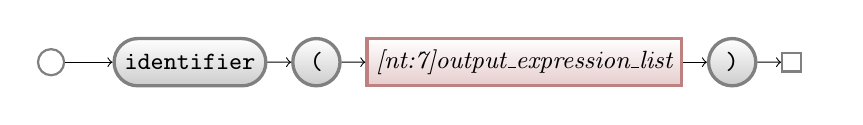
\begin{tikzpicture}
  \matrix[column sep=\ruleMatrixColumnSeparation, row sep=\ruleMatrixRowSeparation] {
    \node (P0start) [firstPoint] {}; & & \node (p0-2) [terminal] {identifier}; & \node (p0-3) [terminal] {(}; & \node (p0-4) [nonterminal] {\nonTerminalSymbol{output\_expression\_list}{7}}; & \node (p0-5) [terminal] {)}; & \node (p0-6) [lastPoint] {}; & \\
  };
  \draw[->] (P0start) -- (p0-2) ;
  \draw[->] (p0-2) -- (p0-3) ;
  \draw[->] (p0-3) -- (p0-4) ;
  \draw[->] (p0-4) -- (p0-5) ;
  \draw[->] (p0-5) -- (p0-6) ;
\end{tikzpicture}

\ruleSubsection{templateSyntax}{templateSyntax}{447}

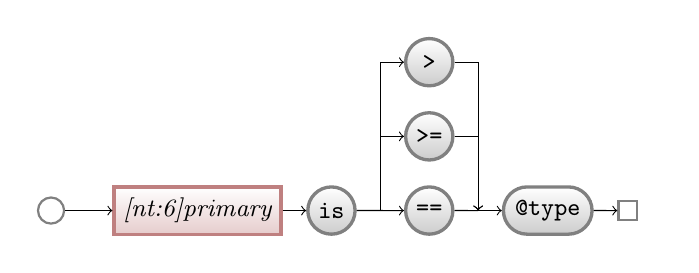
\begin{tikzpicture}
  \matrix[column sep=\ruleMatrixColumnSeparation, row sep=\ruleMatrixRowSeparation] {
    & & & & & \node (p2-5) [terminal] {>}; & \\
    & & & & & \node (p1-5) [terminal] {>=}; & \\
    \node (P0start) [firstPoint] {}; & & \node (p0-2) [nonterminal] {\nonTerminalSymbol{primary}{6}}; & \node (p0-3) [terminal] {is}; & \node (p0-4) [point] {}; & \node (p0-5) [terminal] {==}; & \node (p0-6) [point] {}; & \node (p0-7) [terminal] {@type}; & \node (p0-8) [lastPoint] {}; & \\
  };
  \draw[->] (P0start) -- (p0-2) ;
  \draw[->] (p0-2) -- (p0-3) ;
  \draw[->] (p0-3) -- (p0-5) ;
  \draw[->] (p0-4) |- (p1-5) ;
  \draw[->] (p0-4) |- (p2-5) ;
  \draw (p0-5) -- (p0-6) ;
  \draw[->] (p1-5) -| (p0-6) ;
  \draw[->] (p2-5) -| (p0-6) ;
  \draw[->] (p0-6) -- (p0-7) ;
  \draw[->] (p0-7) -- (p0-8) ;
\end{tikzpicture}

\nonTerminalSection{relation\_factor}{2}

\ruleSubsection{templateSyntax}{templateSyntax}{73}

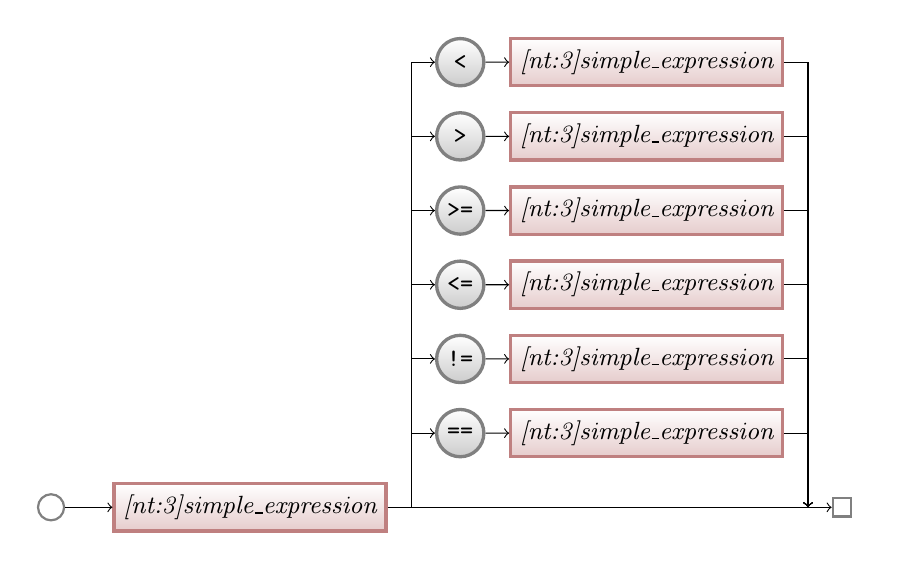
\begin{tikzpicture}
  \matrix[column sep=\ruleMatrixColumnSeparation, row sep=\ruleMatrixRowSeparation] {
    & & & & \node (p6-4) [terminal] {<}; & \node (p6-5) [nonterminal] {\nonTerminalSymbol{simple\_expression}{3}}; & \\
    & & & & \node (p5-4) [terminal] {>}; & \node (p5-5) [nonterminal] {\nonTerminalSymbol{simple\_expression}{3}}; & \\
    & & & & \node (p4-4) [terminal] {>=}; & \node (p4-5) [nonterminal] {\nonTerminalSymbol{simple\_expression}{3}}; & \\
    & & & & \node (p3-4) [terminal] {<=}; & \node (p3-5) [nonterminal] {\nonTerminalSymbol{simple\_expression}{3}}; & \\
    & & & & \node (p2-4) [terminal] {!=}; & \node (p2-5) [nonterminal] {\nonTerminalSymbol{simple\_expression}{3}}; & \\
    & & & & \node (p1-4) [terminal] {==}; & \node (p1-5) [nonterminal] {\nonTerminalSymbol{simple\_expression}{3}}; & \\
    \node (P0start) [firstPoint] {}; & & \node (p0-2) [nonterminal] {\nonTerminalSymbol{simple\_expression}{3}}; & \node (p0-3) [point] {}; & \node (p0-4) [point] {}; & & \node (p0-6) [point] {}; & \node (p0-7) [lastPoint] {}; & \\
  };
  \draw[->] (P0start) -- (p0-2) ;
  \draw (p0-2) -- (p0-4) ;
  \draw[->] (p0-3) |- (p1-4) ;
  \draw[->] (p1-4) -- (p1-5) ;
  \draw[->] (p0-3) |- (p2-4) ;
  \draw[->] (p2-4) -- (p2-5) ;
  \draw[->] (p0-3) |- (p3-4) ;
  \draw[->] (p3-4) -- (p3-5) ;
  \draw[->] (p0-3) |- (p4-4) ;
  \draw[->] (p4-4) -- (p4-5) ;
  \draw[->] (p0-3) |- (p5-4) ;
  \draw[->] (p5-4) -- (p5-5) ;
  \draw[->] (p0-3) |- (p6-4) ;
  \draw[->] (p6-4) -- (p6-5) ;
  \draw (p0-4) -- (p0-6) ;
  \draw[->] (p1-5) -| (p0-6) ;
  \draw[->] (p2-5) -| (p0-6) ;
  \draw[->] (p3-5) -| (p0-6) ;
  \draw[->] (p4-5) -| (p0-6) ;
  \draw[->] (p5-5) -| (p0-6) ;
  \draw[->] (p6-5) -| (p0-6) ;
  \draw[->] (p0-6) -- (p0-7) ;
\end{tikzpicture}

\nonTerminalSection{relation\_term}{1}

\ruleSubsection{templateSyntax}{templateSyntax}{53}

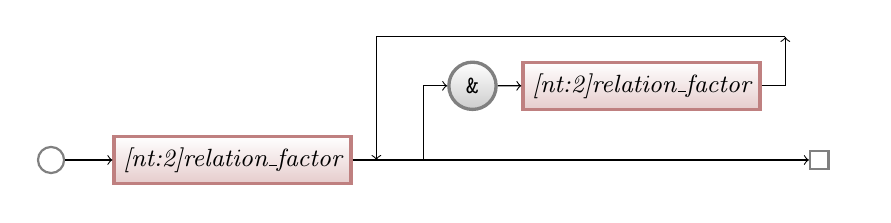
\begin{tikzpicture}
  \matrix[column sep=\ruleMatrixColumnSeparation, row sep=\ruleMatrixRowSeparation] {
    & & & & & & & & \node (p2-8) [point] {}; & \\
    & & & & & & \node (p1-6) [terminal] {\&}; & \node (p1-7) [nonterminal] {\nonTerminalSymbol{relation\_factor}{2}}; & \\
    \node (P0start) [firstPoint] {}; & & \node (p0-2) [nonterminal] {\nonTerminalSymbol{relation\_factor}{2}}; & \node (p0-3) [point] {}; & \node (p0-4) [point] {}; & \node (p0-5) [point] {}; & & & & \node (p0-9) [lastPoint] {}; & \\
  };
  \draw[->] (P0start) -- (p0-2) ;
  \draw (p0-2) -- (p0-4) ;
  \draw[->] (p0-5) |- (p1-6) ;
  \draw[->] (p1-6) -- (p1-7) ;
  \draw[->] (p2-8) -| (p0-3) ;
  \draw[->] (p1-7) -| (p2-8) ;
  \draw[->] (p0-4) -- (p0-9) ;
\end{tikzpicture}

\nonTerminalSection{simple\_expression}{3}

\ruleSubsection{templateSyntax}{templateSyntax}{128}

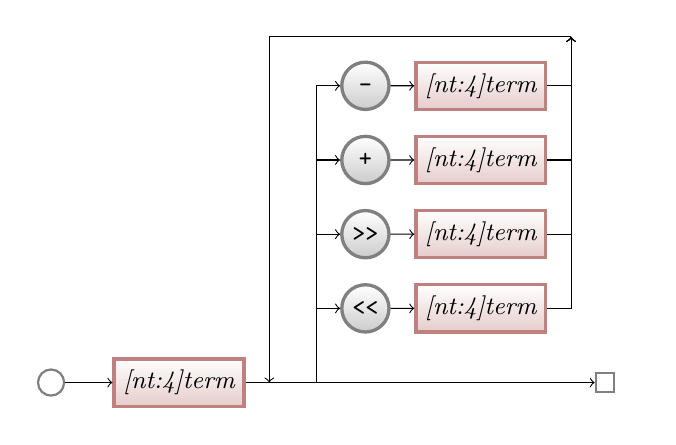
\begin{tikzpicture}
  \matrix[column sep=\ruleMatrixColumnSeparation, row sep=\ruleMatrixRowSeparation] {
    & & & & & & & & \node (p5-8) [point] {}; & \\
    & & & & & & \node (p4-6) [terminal] {-}; & \node (p4-7) [nonterminal] {\nonTerminalSymbol{term}{4}}; & \\
    & & & & & & \node (p3-6) [terminal] {+}; & \node (p3-7) [nonterminal] {\nonTerminalSymbol{term}{4}}; & \\
    & & & & & & \node (p2-6) [terminal] {>>}; & \node (p2-7) [nonterminal] {\nonTerminalSymbol{term}{4}}; & \\
    & & & & & & \node (p1-6) [terminal] {<<}; & \node (p1-7) [nonterminal] {\nonTerminalSymbol{term}{4}}; & \\
    \node (P0start) [firstPoint] {}; & & \node (p0-2) [nonterminal] {\nonTerminalSymbol{term}{4}}; & \node (p0-3) [point] {}; & \node (p0-4) [point] {}; & \node (p0-5) [point] {}; & & & & \node (p0-9) [lastPoint] {}; & \\
  };
  \draw[->] (P0start) -- (p0-2) ;
  \draw (p0-2) -- (p0-4) ;
  \draw[->] (p0-5) |- (p1-6) ;
  \draw[->] (p1-6) -- (p1-7) ;
  \draw[->] (p0-5) |- (p2-6) ;
  \draw[->] (p2-6) -- (p2-7) ;
  \draw[->] (p0-5) |- (p3-6) ;
  \draw[->] (p3-6) -- (p3-7) ;
  \draw[->] (p0-5) |- (p4-6) ;
  \draw[->] (p4-6) -- (p4-7) ;
  \draw[->] (p5-8) -| (p0-3) ;
  \draw[->] (p1-7) -| (p5-8) ;
  \draw[->] (p2-7) -| (p5-8) ;
  \draw[->] (p3-7) -| (p5-8) ;
  \draw[->] (p4-7) -| (p5-8) ;
  \draw[->] (p0-4) -- (p0-9) ;
\end{tikzpicture}

\nonTerminalSection{switch\_case}{12}

\ruleSubsection{templateSyntax}{template-switch-instruction}{61}

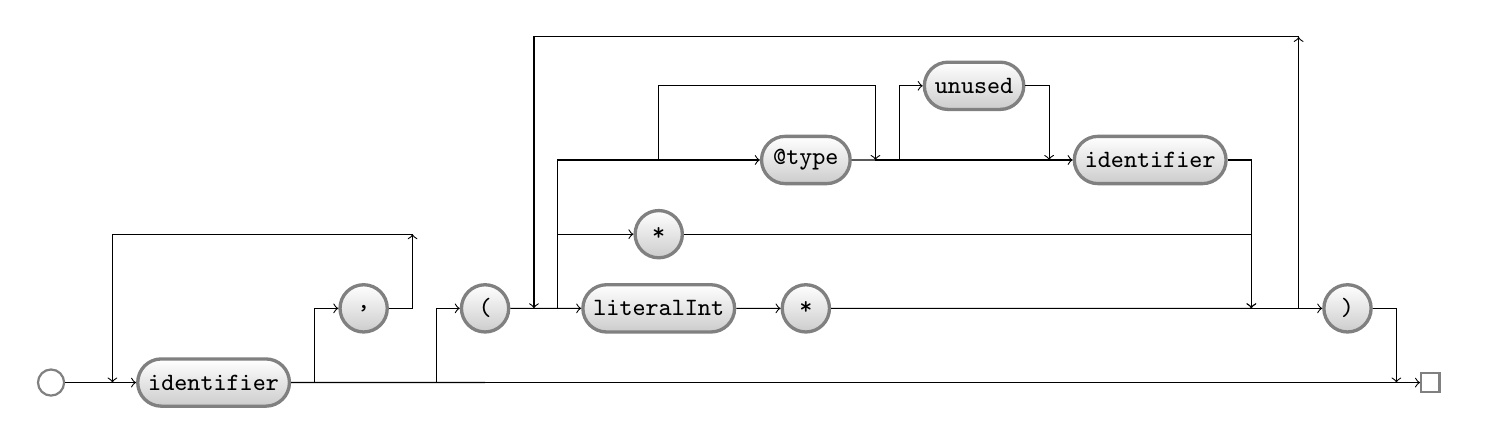
\begin{tikzpicture}
  \matrix[column sep=\ruleMatrixColumnSeparation, row sep=\ruleMatrixRowSeparation] {
    & & & & & & & & & & & & & & & & & & & & \node (p5-20) [point] {}; & \\
    & & & & & & & & & & & & \node (p4-12) [point] {}; & & & \node (p4-15) [terminal] {unused}; & \\
    & & & & & & & & & & & \node (p3-11) [point] {}; & \node (p3-12) [terminal] {@type}; & \node (p3-13) [point] {}; & \node (p3-14) [point] {}; & \node (p3-15) [point] {}; & \node (p3-16) [point] {}; & \node (p3-17) [terminal] {identifier}; & \\
    & & & & & & \node (p2-6) [point] {}; & & & & & \node (p2-11) [terminal] {*}; & \\
    & & & & & \node (p1-5) [terminal] {,}; & & & \node (p1-8) [terminal] {(}; & \node (p1-9) [point] {}; & \node (p1-10) [point] {}; & \node (p1-11) [terminal] {literalInt}; & \node (p1-12) [terminal] {*}; & & & & & & \node (p1-18) [point] {}; & \node (p1-19) [point] {}; & & \node (p1-21) [terminal] {)}; & \\
    \node (P0start) [firstPoint] {}; & & \node (p0-2) [point] {}; & \node (p0-3) [terminal] {identifier}; & \node (p0-4) [point] {}; & & & \node (p0-7) [point] {}; & \node (p0-8) [point] {}; & & & & & & & & & & & & & & \node (p0-22) [point] {}; & \node (p0-23) [lastPoint] {}; & \\
  };
  \draw[->] (P0start) -- (p0-3) ;
  \draw[->] (p0-4) |- (p1-5) ;
  \draw[->] (p2-6) -| (p0-2) ;
  \draw[->] (p1-5) -| (p2-6) ;
  \draw (p0-3) -- (p0-8) ;
  \draw[->] (p0-7) |- (p1-8) ;
  \draw[->] (p1-8) -- (p1-11) ;
  \draw[->] (p1-11) -- (p1-12) ;
  \draw[->] (p1-10) |- (p2-11) ;
  \draw[->] (p1-10) |- (p3-12) ;
  \draw (p3-11) |- (p4-12) ;
  \draw (p3-12) -- (p3-13) ;
  \draw[->] (p4-12) -| (p3-13) ;
  \draw (p3-13) -- (p3-15) ;
  \draw[->] (p3-14) |- (p4-15) ;
  \draw (p3-15) -- (p3-16) ;
  \draw[->] (p4-15) -| (p3-16) ;
  \draw[->] (p3-16) -- (p3-17) ;
  \draw (p1-12) -- (p1-18) ;
  \draw[->] (p2-11) -| (p1-18) ;
  \draw[->] (p3-17) -| (p1-18) ;
  \draw[->] (p5-20) -| (p1-9) ;
  \draw[->] (p1-19) -| (p5-20) ;
  \draw[->] (p1-18) -- (p1-21) ;
  \draw (p0-8) -- (p0-22) ;
  \draw[->] (p1-21) -| (p0-22) ;
  \draw[->] (p0-22) -- (p0-23) ;
\end{tikzpicture}

\nonTerminalSection{template\_instruction}{8}

\ruleSubsection{templateSyntax}{templateSyntax}{493}

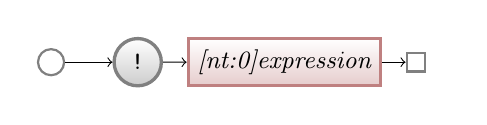
\begin{tikzpicture}
  \matrix[column sep=\ruleMatrixColumnSeparation, row sep=\ruleMatrixRowSeparation] {
    \node (P0start) [firstPoint] {}; & & \node (p0-2) [terminal] {!}; & \node (p0-3) [nonterminal] {\nonTerminalSymbol{expression}{0}}; & \node (p0-4) [lastPoint] {}; & \\
  };
  \draw[->] (P0start) -- (p0-2) ;
  \draw[->] (p0-2) -- (p0-3) ;
  \draw[->] (p0-3) -- (p0-4) ;
\end{tikzpicture}

\ruleSubsection{templateSyntax}{templateSyntax}{505}

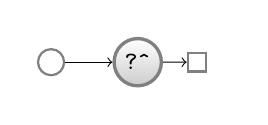
\begin{tikzpicture}
  \matrix[column sep=\ruleMatrixColumnSeparation, row sep=\ruleMatrixRowSeparation] {
    \node (P0start) [firstPoint] {}; & & \node (p0-2) [terminal] {?\verb=^=}; & \node (p0-3) [lastPoint] {}; & \\
  };
  \draw[->] (P0start) -- (p0-2) ;
  \draw[->] (p0-2) -- (p0-3) ;
\end{tikzpicture}

\ruleSubsection{templateSyntax}{templateSyntax}{512}

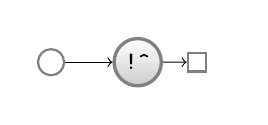
\begin{tikzpicture}
  \matrix[column sep=\ruleMatrixColumnSeparation, row sep=\ruleMatrixRowSeparation] {
    \node (P0start) [firstPoint] {}; & & \node (p0-2) [terminal] {!\verb=^=}; & \node (p0-3) [lastPoint] {}; & \\
  };
  \draw[->] (P0start) -- (p0-2) ;
  \draw[->] (p0-2) -- (p0-3) ;
\end{tikzpicture}

\ruleSubsection{templateSyntax}{templateSyntax}{519}

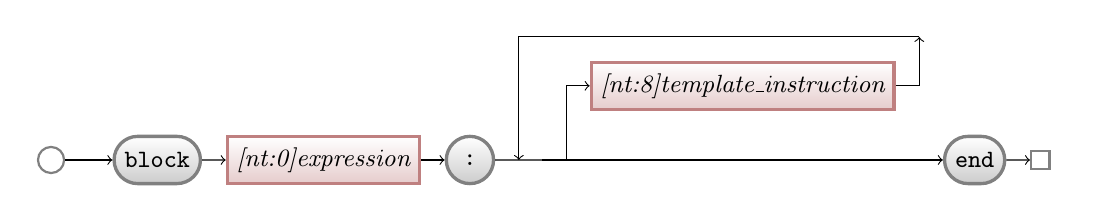
\begin{tikzpicture}
  \matrix[column sep=\ruleMatrixColumnSeparation, row sep=\ruleMatrixRowSeparation] {
    & & & & & & & & & \node (p2-9) [point] {}; & \\
    & & & & & & & & \node (p1-8) [nonterminal] {\nonTerminalSymbol{template\_instruction}{8}}; & \\
    \node (P0start) [firstPoint] {}; & & \node (p0-2) [terminal] {block}; & \node (p0-3) [nonterminal] {\nonTerminalSymbol{expression}{0}}; & \node (p0-4) [terminal] {:}; & \node (p0-5) [point] {}; & \node (p0-6) [point] {}; & \node (p0-7) [point] {}; & & & \node (p0-10) [terminal] {end}; & \node (p0-11) [lastPoint] {}; & \\
  };
  \draw[->] (P0start) -- (p0-2) ;
  \draw[->] (p0-2) -- (p0-3) ;
  \draw[->] (p0-3) -- (p0-4) ;
  \draw (p0-4) -- (p0-6) ;
  \draw[->] (p0-7) |- (p1-8) ;
  \draw[->] (p2-9) -| (p0-5) ;
  \draw[->] (p1-8) -| (p2-9) ;
  \draw[->] (p0-6) -- (p0-10) ;
  \draw[->] (p0-10) -- (p0-11) ;
\end{tikzpicture}

\ruleSubsection{templateSyntax}{templateSyntax}{540}

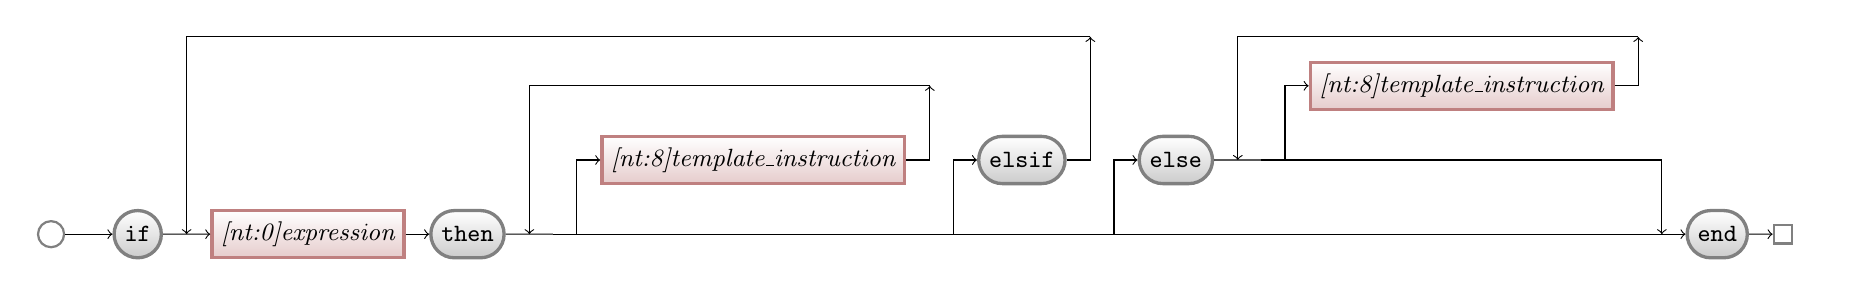
\begin{tikzpicture}
  \matrix[column sep=\ruleMatrixColumnSeparation, row sep=\ruleMatrixRowSeparation] {
    & & & & & & & & & & & & & \node (p3-13) [point] {}; & & & & & & & \node (p3-20) [point] {}; & \\
    & & & & & & & & & & \node (p2-10) [point] {}; & & & & & & & & & \node (p2-19) [nonterminal] {\nonTerminalSymbol{template\_instruction}{8}}; & \\
    & & & & & & & & & \node (p1-9) [nonterminal] {\nonTerminalSymbol{template\_instruction}{8}}; & & & \node (p1-12) [terminal] {elsif}; & & & \node (p1-15) [terminal] {else}; & \node (p1-16) [point] {}; & \node (p1-17) [point] {}; & \node (p1-18) [point] {}; & \\
    \node (P0start) [firstPoint] {}; & & \node (p0-2) [terminal] {if}; & \node (p0-3) [point] {}; & \node (p0-4) [nonterminal] {\nonTerminalSymbol{expression}{0}}; & \node (p0-5) [terminal] {then}; & \node (p0-6) [point] {}; & \node (p0-7) [point] {}; & \node (p0-8) [point] {}; & & & \node (p0-11) [point] {}; & & & \node (p0-14) [point] {}; & \node (p0-15) [point] {}; & & & & & & \node (p0-21) [point] {}; & \node (p0-22) [terminal] {end}; & \node (p0-23) [lastPoint] {}; & \\
  };
  \draw[->] (P0start) -- (p0-2) ;
  \draw[->] (p0-2) -- (p0-4) ;
  \draw[->] (p0-4) -- (p0-5) ;
  \draw (p0-5) -- (p0-7) ;
  \draw[->] (p0-8) |- (p1-9) ;
  \draw[->] (p2-10) -| (p0-6) ;
  \draw[->] (p1-9) -| (p2-10) ;
  \draw[->] (p0-11) |- (p1-12) ;
  \draw[->] (p3-13) -| (p0-3) ;
  \draw[->] (p1-12) -| (p3-13) ;
  \draw (p0-7) -- (p0-15) ;
  \draw[->] (p0-14) |- (p1-15) ;
  \draw (p1-15) -- (p1-17) ;
  \draw[->] (p1-18) |- (p2-19) ;
  \draw[->] (p3-20) -| (p1-16) ;
  \draw[->] (p2-19) -| (p3-20) ;
  \draw (p0-15) -- (p0-21) ;
  \draw[->] (p1-17) -| (p0-21) ;
  \draw[->] (p0-21) -- (p0-22) ;
  \draw[->] (p0-22) -- (p0-23) ;
\end{tikzpicture}

\ruleSubsection{templateSyntax}{template-for-instruction}{106}

\begin{tikzpicture}
  \matrix[column sep=\ruleMatrixColumnSeparation, row sep=\ruleMatrixRowSeparation] {
    & & & & & & & & & & & & & \node (p3-13) [point] {}; & & & & & & & & & & & & & & & & & & & \node (p3-32) [point] {}; & & & & & & & & \node (p3-40) [point] {}; & \\
    & & & & \node (p2-4) [terminal] {>}; & & & & & & & & \node (p2-12) [nonterminal] {\nonTerminalSymbol{template\_instruction}{8}}; & & & & & & & & & & & & & \node (p2-25) [point] {}; & & & & & & \node (p2-31) [nonterminal] {\nonTerminalSymbol{template\_instruction}{8}}; & & & & & & & & \node (p2-39) [nonterminal] {\nonTerminalSymbol{template\_instruction}{8}}; & \\
    & & & & \node (p1-4) [terminal] {<}; & & & & \node (p1-8) [terminal] {before}; & \node (p1-9) [point] {}; & \node (p1-10) [point] {}; & \node (p1-11) [point] {}; & & & & & & \node (p1-17) [terminal] {(}; & \node (p1-18) [terminal] {identifier}; & \node (p1-19) [terminal] {)}; & & & & & \node (p1-24) [nonterminal] {\nonTerminalSymbol{template\_instruction}{8}}; & & & \node (p1-27) [terminal] {between}; & \node (p1-28) [point] {}; & \node (p1-29) [point] {}; & \node (p1-30) [point] {}; & & & & & \node (p1-35) [terminal] {after}; & \node (p1-36) [point] {}; & \node (p1-37) [point] {}; & \node (p1-38) [point] {}; & \\
    \node (P0start) [firstPoint] {}; & & \node (p0-2) [terminal] {for}; & \node (p0-3) [point] {}; & \node (p0-4) [point] {}; & \node (p0-5) [point] {}; & \node (p0-6) [nonterminal] {\nonTerminalSymbol{for\_instruction\_enumerated\_object}{11}}; & \node (p0-7) [point] {}; & \node (p0-8) [point] {}; & & & & & & \node (p0-14) [point] {}; & \node (p0-15) [terminal] {do}; & \node (p0-16) [point] {}; & \node (p0-17) [point] {}; & & & \node (p0-20) [point] {}; & \node (p0-21) [point] {}; & \node (p0-22) [point] {}; & \node (p0-23) [point] {}; & & & \node (p0-26) [point] {}; & \node (p0-27) [point] {}; & & & & & & \node (p0-33) [point] {}; & \node (p0-34) [point] {}; & \node (p0-35) [point] {}; & & & & & & \node (p0-41) [point] {}; & \node (p0-42) [terminal] {end}; & \node (p0-43) [lastPoint] {}; & \\
  };
  \draw[->] (P0start) -- (p0-2) ;
  \draw (p0-2) -- (p0-4) ;
  \draw[->] (p0-3) |- (p1-4) ;
  \draw[->] (p0-3) |- (p2-4) ;
  \draw (p0-4) -- (p0-5) ;
  \draw[->] (p1-4) -| (p0-5) ;
  \draw[->] (p2-4) -| (p0-5) ;
  \draw[->] (p0-5) -- (p0-6) ;
  \draw (p0-6) -- (p0-8) ;
  \draw[->] (p0-7) |- (p1-8) ;
  \draw (p1-8) -- (p1-10) ;
  \draw[->] (p1-11) |- (p2-12) ;
  \draw[->] (p3-13) -| (p1-9) ;
  \draw[->] (p2-12) -| (p3-13) ;
  \draw (p0-8) -- (p0-14) ;
  \draw[->] (p1-10) -| (p0-14) ;
  \draw[->] (p0-14) -- (p0-15) ;
  \draw (p0-15) -- (p0-17) ;
  \draw[->] (p0-16) |- (p1-17) ;
  \draw[->] (p1-17) -- (p1-18) ;
  \draw[->] (p1-18) -- (p1-19) ;
  \draw (p0-17) -- (p0-20) ;
  \draw[->] (p1-19) -| (p0-20) ;
  \draw (p0-20) -- (p0-22) ;
  \draw[->] (p0-23) |- (p1-24) ;
  \draw[->] (p2-25) -| (p0-21) ;
  \draw[->] (p1-24) -| (p2-25) ;
  \draw (p0-22) -- (p0-27) ;
  \draw[->] (p0-26) |- (p1-27) ;
  \draw (p1-27) -- (p1-29) ;
  \draw[->] (p1-30) |- (p2-31) ;
  \draw[->] (p3-32) -| (p1-28) ;
  \draw[->] (p2-31) -| (p3-32) ;
  \draw (p0-27) -- (p0-33) ;
  \draw[->] (p1-29) -| (p0-33) ;
  \draw (p0-33) -- (p0-35) ;
  \draw[->] (p0-34) |- (p1-35) ;
  \draw (p1-35) -- (p1-37) ;
  \draw[->] (p1-38) |- (p2-39) ;
  \draw[->] (p3-40) -| (p1-36) ;
  \draw[->] (p2-39) -| (p3-40) ;
  \draw (p0-35) -- (p0-41) ;
  \draw[->] (p1-37) -| (p0-41) ;
  \draw[->] (p0-41) -- (p0-42) ;
  \draw[->] (p0-42) -- (p0-43) ;
\end{tikzpicture}

\ruleSubsection{templateSyntax}{template-switch-instruction}{28}

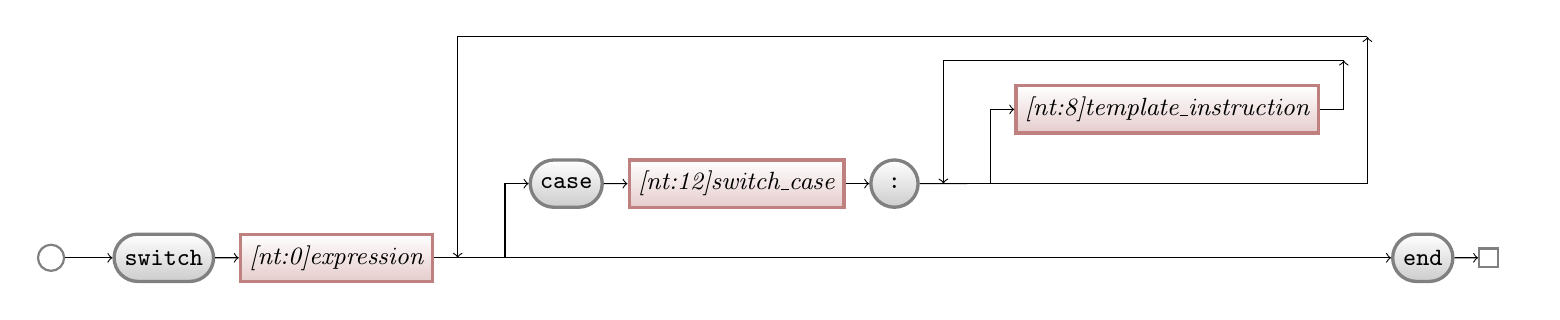
\begin{tikzpicture}
  \matrix[column sep=\ruleMatrixColumnSeparation, row sep=\ruleMatrixRowSeparation] {
    & & & & & & & & & & & & & & & \node (p4-15) [point] {}; & \\
    & & & & & & & & & & & & & & \node (p3-14) [point] {}; & \\
    & & & & & & & & & & & & & \node (p2-13) [nonterminal] {\nonTerminalSymbol{template\_instruction}{8}}; & \\
    & & & & & & & \node (p1-7) [terminal] {case}; & \node (p1-8) [nonterminal] {\nonTerminalSymbol{switch\_case}{12}}; & \node (p1-9) [terminal] {:}; & \node (p1-10) [point] {}; & \node (p1-11) [point] {}; & \node (p1-12) [point] {}; & \\
    \node (P0start) [firstPoint] {}; & & \node (p0-2) [terminal] {switch}; & \node (p0-3) [nonterminal] {\nonTerminalSymbol{expression}{0}}; & \node (p0-4) [point] {}; & \node (p0-5) [point] {}; & \node (p0-6) [point] {}; & & & & & & & & & & \node (p0-16) [terminal] {end}; & \node (p0-17) [lastPoint] {}; & \\
  };
  \draw[->] (P0start) -- (p0-2) ;
  \draw[->] (p0-2) -- (p0-3) ;
  \draw (p0-3) -- (p0-5) ;
  \draw[->] (p0-6) |- (p1-7) ;
  \draw[->] (p1-7) -- (p1-8) ;
  \draw[->] (p1-8) -- (p1-9) ;
  \draw (p1-9) -- (p1-11) ;
  \draw[->] (p1-12) |- (p2-13) ;
  \draw[->] (p3-14) -| (p1-10) ;
  \draw[->] (p2-13) -| (p3-14) ;
  \draw[->] (p4-15) -| (p0-4) ;
  \draw[->] (p1-11) -| (p4-15) ;
  \draw[->] (p0-5) -- (p0-16) ;
  \draw[->] (p0-16) -- (p0-17) ;
\end{tikzpicture}

\nonTerminalSection{template\_parser\_start\_symbol}{9}

\ruleSubsection{templateSyntax}{templateSyntax}{576}

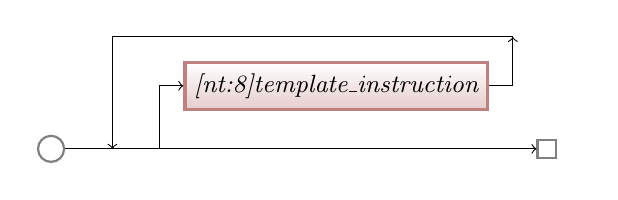
\begin{tikzpicture}
  \matrix[column sep=\ruleMatrixColumnSeparation, row sep=\ruleMatrixRowSeparation] {
    & & & & & & \node (p2-6) [point] {}; & \\
    & & & & & \node (p1-5) [nonterminal] {\nonTerminalSymbol{template\_instruction}{8}}; & \\
    \node (P0start) [firstPoint] {}; & & \node (p0-2) [point] {}; & \node (p0-3) [point] {}; & \node (p0-4) [point] {}; & & & \node (p0-7) [lastPoint] {}; & \\
  };
  \draw (P0start) -- (p0-3) ;
  \draw[->] (p0-4) |- (p1-5) ;
  \draw[->] (p2-6) -| (p0-2) ;
  \draw[->] (p1-5) -| (p2-6) ;
  \draw[->] (p0-3) -- (p0-7) ;
\end{tikzpicture}

\nonTerminalSection{term}{4}

\ruleSubsection{templateSyntax}{templateSyntax}{168}

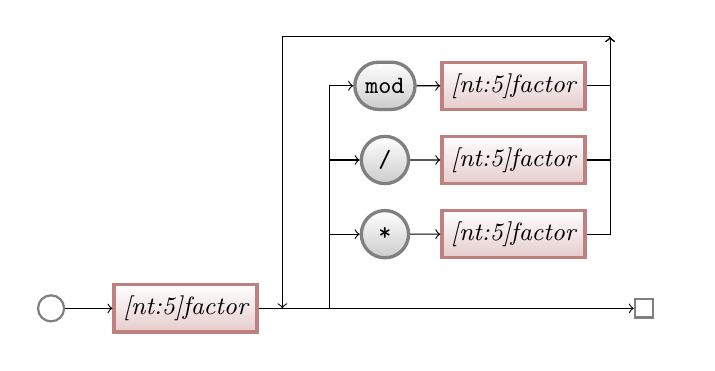
\begin{tikzpicture}
  \matrix[column sep=\ruleMatrixColumnSeparation, row sep=\ruleMatrixRowSeparation] {
    & & & & & & & & \node (p4-8) [point] {}; & \\
    & & & & & & \node (p3-6) [terminal] {mod}; & \node (p3-7) [nonterminal] {\nonTerminalSymbol{factor}{5}}; & \\
    & & & & & & \node (p2-6) [terminal] {/}; & \node (p2-7) [nonterminal] {\nonTerminalSymbol{factor}{5}}; & \\
    & & & & & & \node (p1-6) [terminal] {*}; & \node (p1-7) [nonterminal] {\nonTerminalSymbol{factor}{5}}; & \\
    \node (P0start) [firstPoint] {}; & & \node (p0-2) [nonterminal] {\nonTerminalSymbol{factor}{5}}; & \node (p0-3) [point] {}; & \node (p0-4) [point] {}; & \node (p0-5) [point] {}; & & & & \node (p0-9) [lastPoint] {}; & \\
  };
  \draw[->] (P0start) -- (p0-2) ;
  \draw (p0-2) -- (p0-4) ;
  \draw[->] (p0-5) |- (p1-6) ;
  \draw[->] (p1-6) -- (p1-7) ;
  \draw[->] (p0-5) |- (p2-6) ;
  \draw[->] (p2-6) -- (p2-7) ;
  \draw[->] (p0-5) |- (p3-6) ;
  \draw[->] (p3-6) -- (p3-7) ;
  \draw[->] (p4-8) -| (p0-3) ;
  \draw[->] (p1-7) -| (p4-8) ;
  \draw[->] (p2-7) -| (p4-8) ;
  \draw[->] (p3-7) -| (p4-8) ;
  \draw[->] (p0-4) -- (p0-9) ;
\end{tikzpicture}



\end{document}
